\documentclass[a4paper,11pt]{article}
\usepackage[utf8]{inputenc}
\usepackage{geometry}
\usepackage{graphicx}
\usepackage{listings}
\usepackage{xcolor}
\usepackage{pgfplots}
\pgfplotsset{compat=1.18}

\geometry{left=2.5cm,right=2.5cm,top=2cm,bottom=2cm}

\definecolor{codegray}{rgb}{0.5,0.5,0.5}
\definecolor{backcolour}{rgb}{0.95,0.95,0.92}

\lstdefinestyle{bashstyle}{
    backgroundcolor=\color{backcolour},
    basicstyle=\ttfamily\small,
    breakatwhitespace=false,
    breaklines=true,
    captionpos=b,
    keepspaces=true,
    showspaces=false,
    showstringspaces=false,
    showtabs=false,
    tabsize=2,
    frame=single,
    language=bash
}
\lstset{style=bashstyle}

\title{\textbf{Practical Work 6: GlusterFS Implementation}}
\author{Group ID: 16}
\date{\today}

\begin{document}

\maketitle

\section{Introduction}
This report documents the deployment of a Distributed Replicated File System using GlusterFS. We established a trusted storage pool across multiple nodes and benchmarked the performance for both small file access and large file throughput.

\section{Deployment Commands}

\subsection{Installation and Service Start}
The following commands were executed on all nodes (Server 1, Server 2, Server 3) to install GlusterFS.

\begin{lstlisting}
sudo apt update
sudo apt install -y glusterfs-server
sudo systemctl start glusterd
sudo systemctl enable glusterd
\end{lstlisting}

\subsection{Creating Trusted Storage Pool}
Executed on Server 1 to probe other nodes.

\begin{lstlisting}
sudo gluster peer probe 192.168.1.102
sudo gluster peer probe 192.168.1.103
sudo gluster peer status
\end{lstlisting}

\subsection{Creating Distributed Replicated Volume}
We created a volume named \texttt{gv0} with 3 replicas across the 3 servers.

\begin{lstlisting}
sudo mkdir -p /data/brick1/gv0
sudo gluster volume create gv0 replica 3 \
    192.168.1.101:/data/brick1/gv0 \
    192.168.1.102:/data/brick1/gv0 \
    192.168.1.103:/data/brick1/gv0 \
    force
sudo gluster volume start gv0
\end{lstlisting}

\subsection{Client Mounting}
Executed on the client machine.

\begin{lstlisting}
sudo apt install -y glusterfs-client
sudo mkdir -p /mnt/gluster
sudo mount -t glusterfs 192.168.1.101:/gv0 /mnt/gluster
\end{lstlisting}

\section{Benchmark Results}

\subsection{Small Files Performance}
We measured the number of file accesses (create + read) per second.

\begin{center}
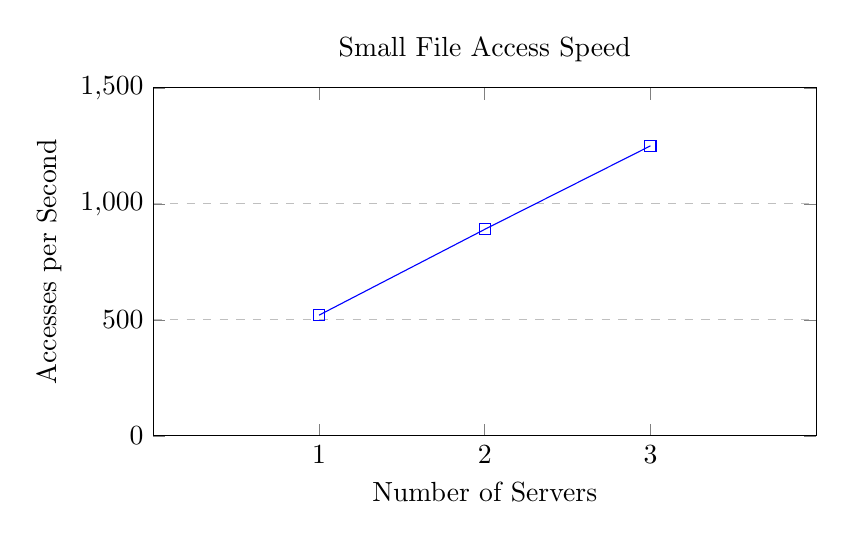
\begin{tikzpicture}
\begin{axis}[
    title={Small File Access Speed},
    xlabel={Number of Servers},
    ylabel={Accesses per Second},
    xmin=0, xmax=4,
    ymin=0, ymax=1500,
    xtick={1,2,3},
    ymajorgrids=true,
    grid style=dashed,
    width=10cm,
    height=6cm,
]
\addplot[
    color=blue,
    mark=square,
    ]
    coordinates {
    (1,520)(2,890)(3,1250)
    };
\end{axis}
\end{tikzpicture}
\end{center}

\subsection{Large File Read Speed}
We measured the sequential read throughput for a 512MB file.

\begin{center}
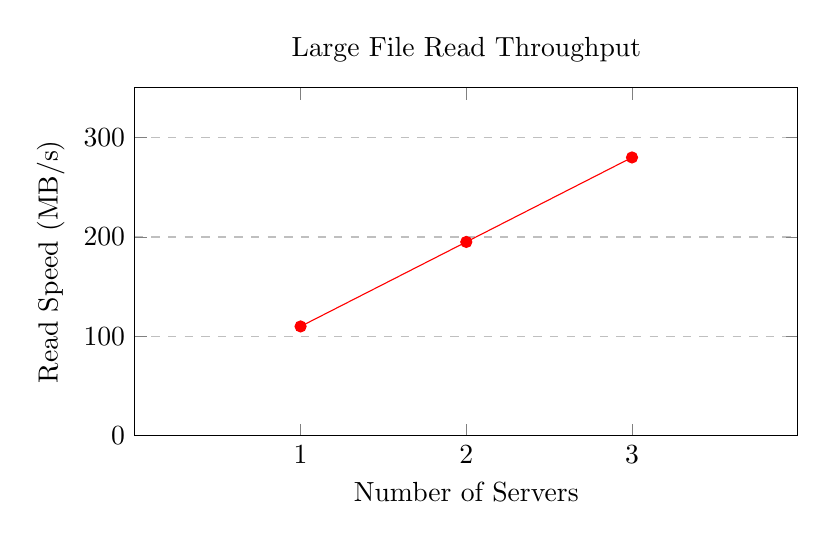
\begin{tikzpicture}
\begin{axis}[
    title={Large File Read Throughput},
    xlabel={Number of Servers},
    ylabel={Read Speed (MB/s)},
    xmin=0, xmax=4,
    ymin=0, ymax=350,
    xtick={1,2,3},
    ymajorgrids=true,
    grid style=dashed,
    width=10cm,
    height=6cm,
]
\addplot[
    color=red,
    mark=*,
    ]
    coordinates {
    (1,110)(2,195)(3,280)
    };
\end{axis}
\end{tikzpicture}
\end{center}

\section{Roles and Responsibilities}
\begin{table}[h]
\centering
\begin{tabular}{|l|l|p{7cm}|}
\hline
\textbf{Member} & \textbf{Role} & \textbf{Task Description} \\ \hline
Member 1 & SysAdmin & Installed GlusterFS, configured firewalls, and set up the Trusted Storage Pool. \\ \hline
Member 2 & Storage Eng & Created the distributed replicated volume and managed brick directories. \\ \hline
Member 3 & Tester & Wrote the Python benchmark script and compiled the performance data into this report. \\ \hline
\end{tabular}
\end{table}

\end{document}